%%%%%%%%%%%%%%%%%%%%%%%%%%%%%%%%%%%%%%%%%%%%%%%%%%
\section{Detector Calibration}
%%%%%%%%%%%%%%%%%%%%%%%%%%%%%%%%%%%%%%%%%%%%%%%%%%

%%%%%%%%%%%%%%%%%%%%%%%%%%%%%%%%%%%%%%%%%%%%%%%%%%
\subsection{Channel-by-Channel Calibration}
%%%%%%%%%%%%%%%%%%%%%%%%%%%%%%%%%%%%%%%%%%%%%%%%%%

Figure~\ref{fig:PionQvsCh} shows the hit charge as a function of 
the TPC channel number obtained from the 800 MeV/$c$ $\pi^+$ data. 
This figure is obtained from $\sim$300 events of well-selected Pion passing-through the TPC.
Gray-scale contours show hit charge distributions for
each channel and black points correspond to average of the hit charge distribution.  
Although we expect the energy deposition of the through-going pion to be uniform,
we observe relatively large channel dependence. 
This is mainly because of the distortion of the TPC drift field.
We use this average charge as channel-by-channel normalization scale.

\begin{figure}[htbp]
 \begin{center}
%  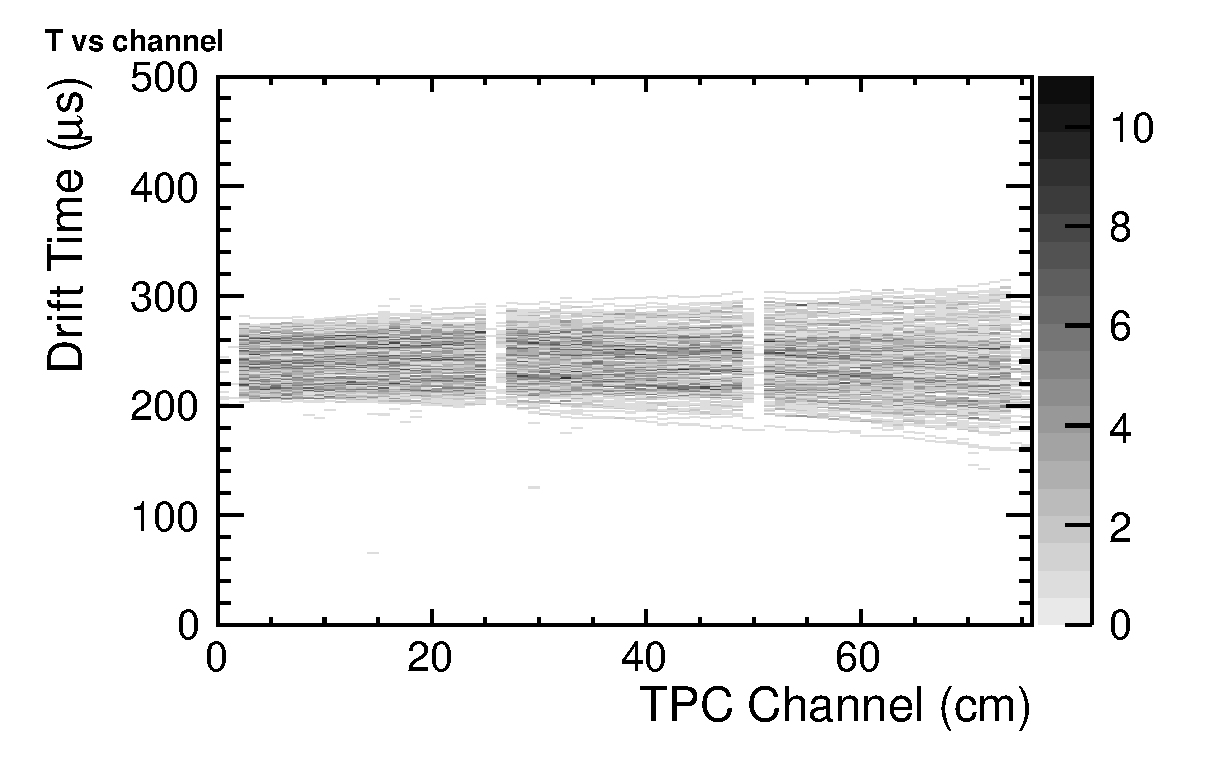
\includegraphics[width=0.8\hsize]{fig/PionTrack.eps}
  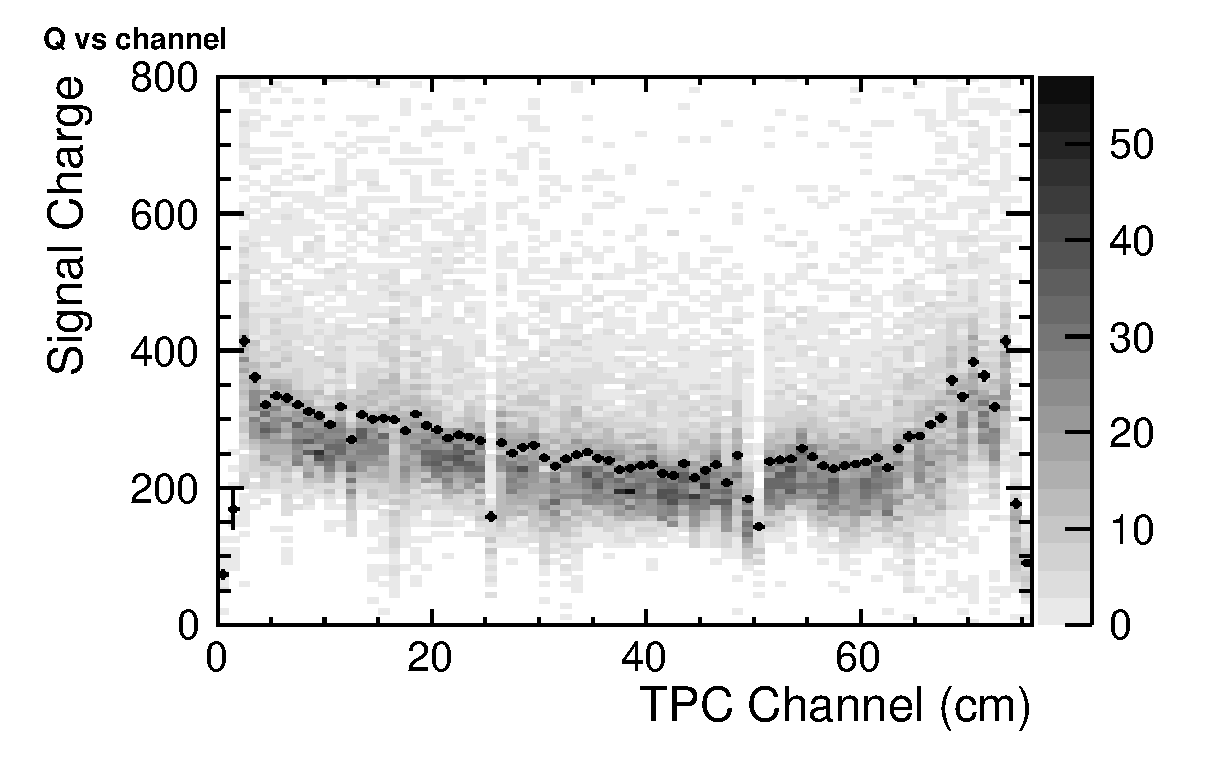
\includegraphics[width=1.0\hsize]{fig/PionQvsCh.eps}
 \end{center}
 \caption{800 MeV/c pion average hit charge}
 \label{fig:PionQvsCh}
\end{figure}

Figure~\ref{Fig:FieldLine} shows line of force around anode  calculated using 
a 2D FEM (Finite Element Method) package \cite{Ref:FEMTET},
where horizontal axis and vertical axis correspond to the beam line direction and 
the drift direction, respectively.
Anode and grid are located at TPC height =20 cm and 21 cm, respectively.
Top plot shows the field around corner of the TPC
and bottom plot is around suport frame of the grid plane.
There are significant distortion of the electric field.
We found this field distortion is the main cause of the
non-uniformity of the TPC response.

%\begin{figure}[htbp]
% \begin{center}
%  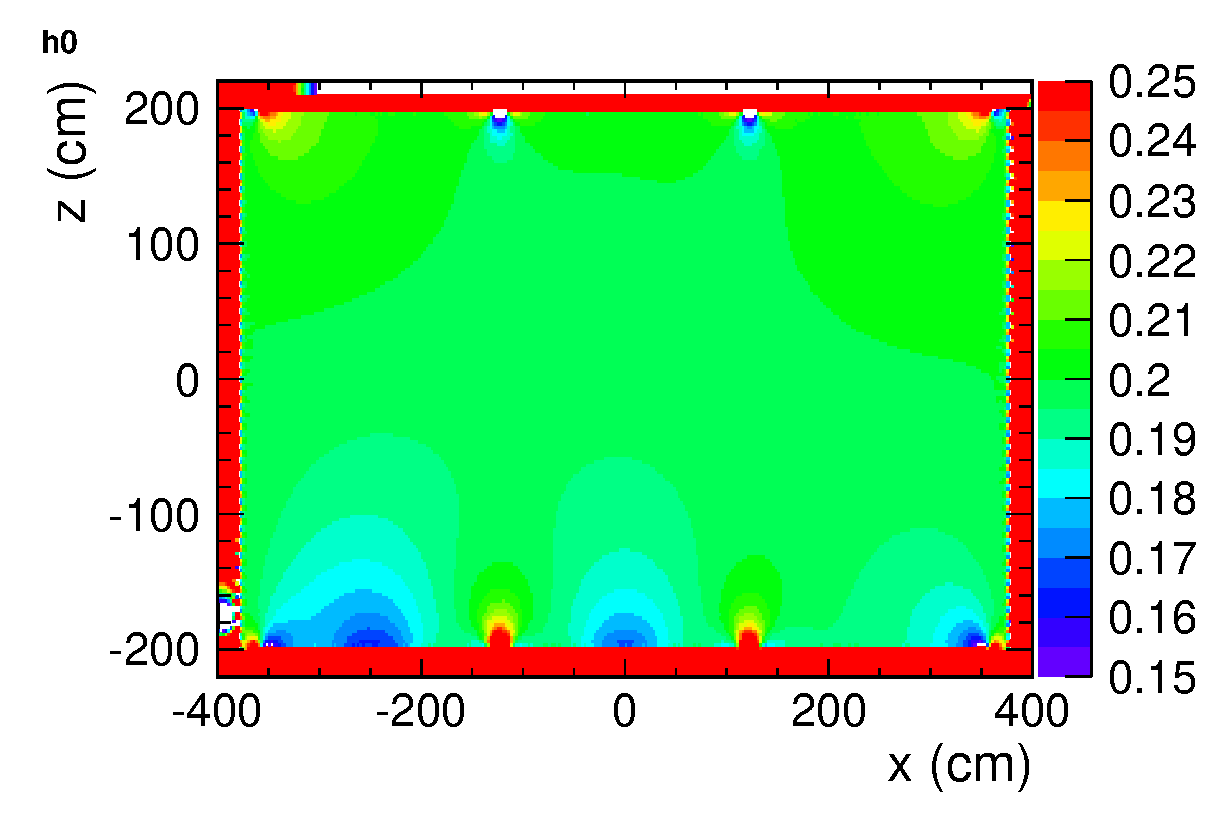
\includegraphics[width=1.0\hsize]{fig/2DFieldMap.eps}
% \end{center}
% \caption{Electric field map obtained with 2D FEM where
%horizontal axis corresponds to the beam line direction,
%and vertical axis corresponds to drift direction,
%and color strength corresponds to electric field strength in V/cm.
%}
% \label{Fig:2DFieldMap}
%\end{figure}

\begin{figure}[htbp]
 \begin{center}
  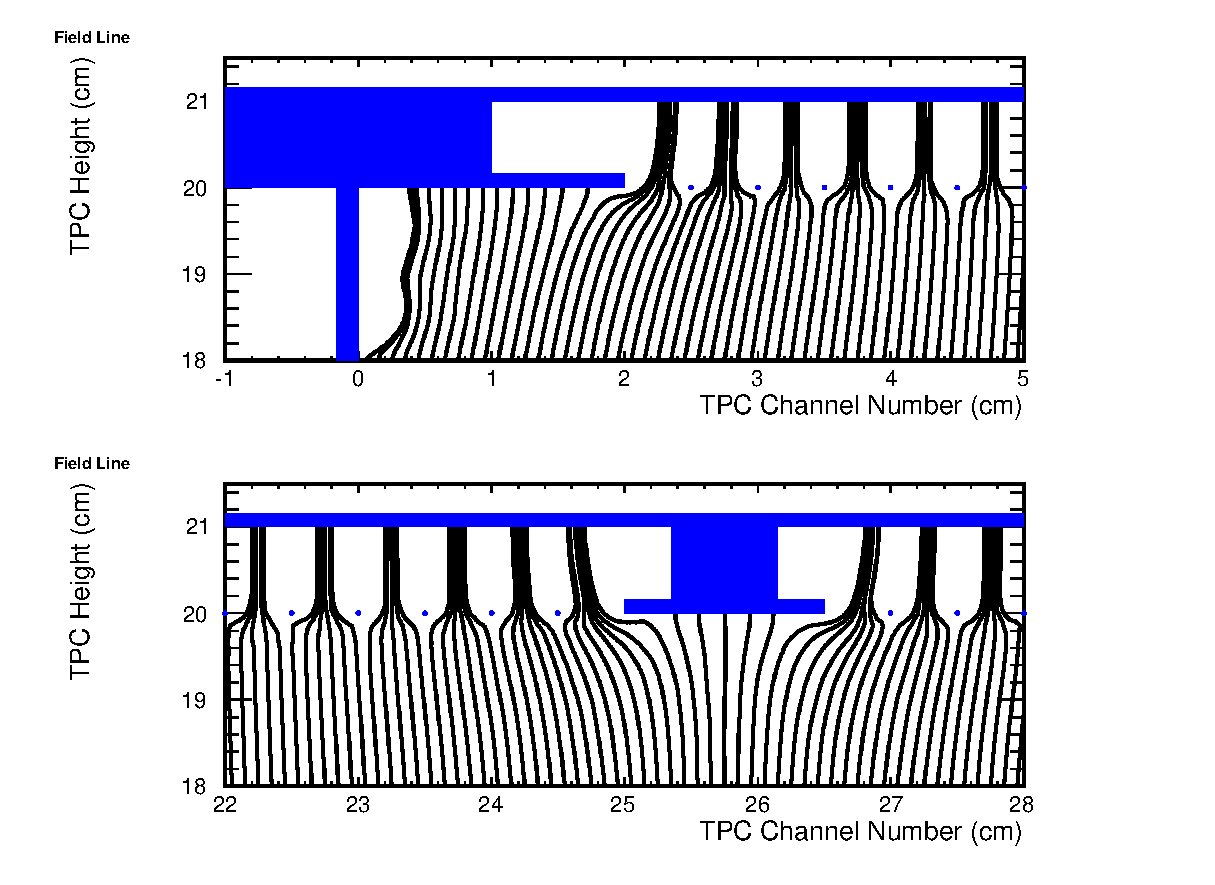
\includegraphics[width=1.0\hsize]{fig/FieldLine.eps}
 \end{center}
 \caption{Line of force of the electric field obtained with 
2D FEM where horizontal axis corresponds to the beam line direction,
and vertical axis corresponds to drift direction.
}
 \label{Fig:FieldLine}
\end{figure}

%%%%%%%%%%%%%%%%%%%%%%%%%%%%%%%%%%%%%%%%%%%%%%%%%%
\subsection{Liquid Argon Purity}
%%%%%%%%%%%%%%%%%%%%%%%%%%%%%%%%%%%%%%%%%%%%%%%%%%

Attenuation of the drift electron depends on purity of LAr since electronegative impurities capture it \cite{purity}. 
Thus we need to apply correction to TPC signal charge according to the drift time.
We use cosmic ray events triggered by inner PMT at off-beam timing for measuring the LAr purity, and use this to correct the beam data.
Figure~\ref{fig:CosmicEvent} shows an event display of typical cosmic muon event crossing TPC channels.
The attenuation of readout charge depending on drift time is clearly seen in the right plot. 
We use multiple events to cancel Landau effect and apply channel response correction to estimate LAr purity.

\begin{figure}[htbp]
 \begin{center}
  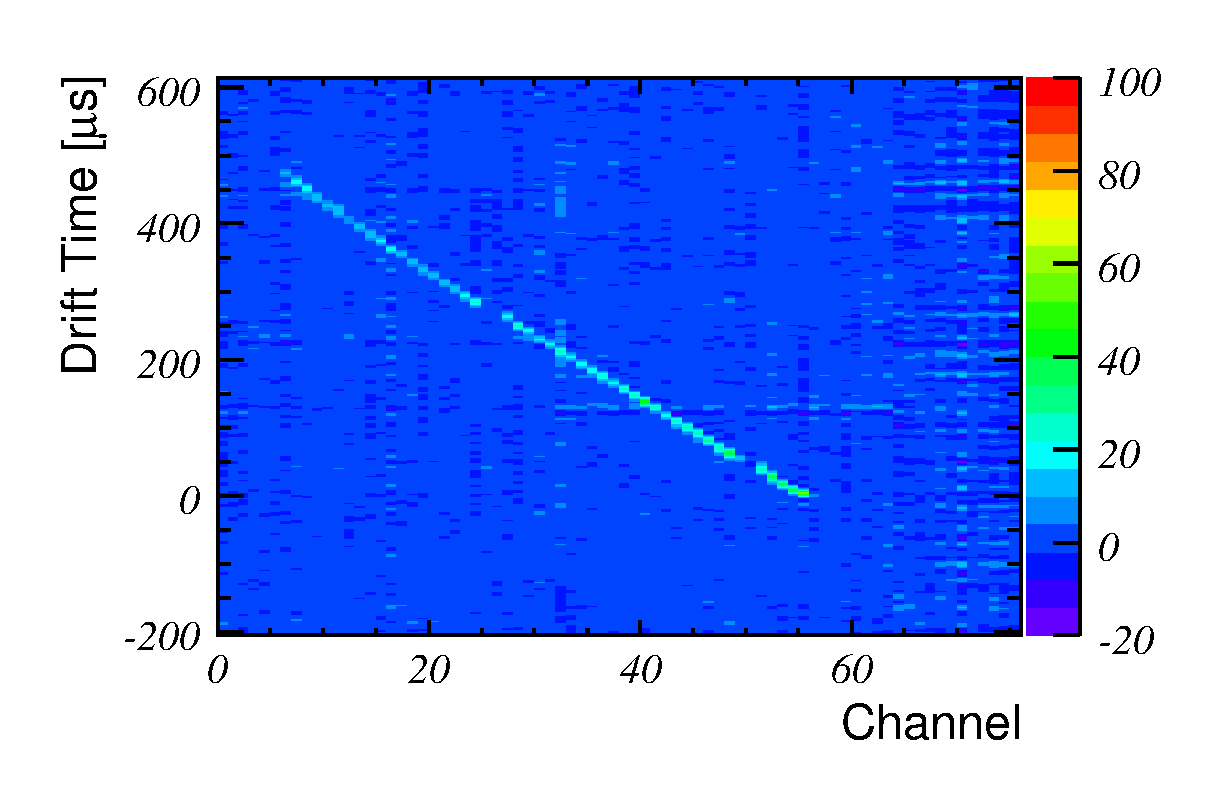
\includegraphics[width=0.49\hsize]{fig/cosmic68_ev258_display.eps}
  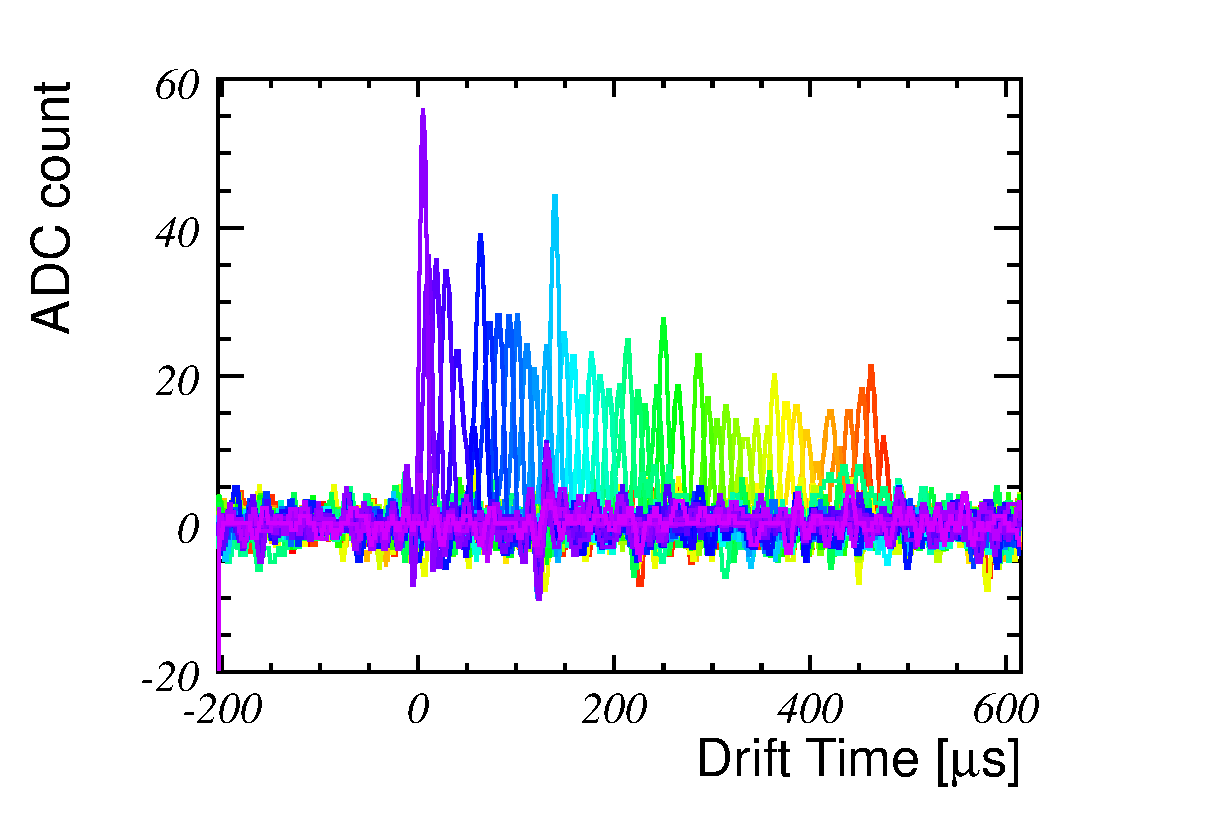
\includegraphics[width=0.49\hsize]{fig/cosmic68_ev258.eps}
 \end{center}
 \caption{Left: Typical cosmic muon event crossing TPC channels. Right: Charge deposit as a function of drift time.}
 \label{fig:CosmicEvent}
\end{figure}

We select cosmic ray event with more than 20 TPC channels which corresponds to zenith angle of more than $27^\circ$ and consistent with straight line by $\chi^2$ fit. 
%Readout charge is corrected for field distortion and projected to beam direction to correct injection angle.
We fit readout charge by Landau function in each drift time bin to estimate average charge deposit. 
%Figure~\ref{fig:tauExample} shows example of the average readout charge as a function of drift time which is fitted by exponential to obtain drift electron lifetime. 
%Realistic Monte Carlo simulation shows about 13\% (TBU) smaller lifetime estimation due to noise, field distortion, and FFT effects. 
%We correct output lifetime from these effects.
Figure~\ref{fig:CosmicPurity} shows an drift electron lifetime as a function of duration after initial LAr filling.
Drift electron lifetime was 600 $\mu$s at 60 hours, and 400 $\mu$s after 150 hours.
%Initial purity looks good, but the purity was slowly degrading while data taking period.
The degradation is possibly due to impurity from micro leak or out-gassing penetrating faster than purification by gas recirculation.
But we kept enough drift electron lifetime during data taking period.
The effects from noise, field distortion, and FFT give about 10\% (to be confirmed) of systematic uncertainty in LAr purity estimation.
%Since charge in simulation is calibrated using through-going $\pi$ data as described later and duration of analyzed beam data is short (about 30 hours), this uncertainty gives negligible effects (to be updated, show percentage) in beam data analysis. 

%\begin{figure}[htbp]
% \begin{center}
%  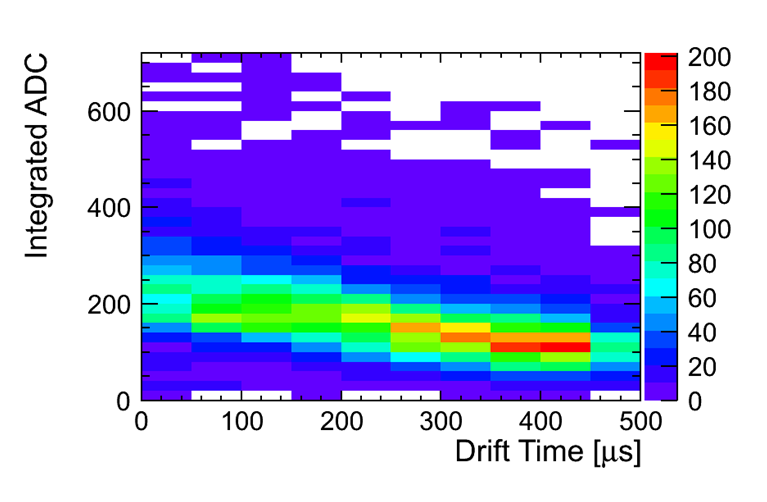
\includegraphics[width=0.45\hsize]{fig/chargeDep.eps}
%  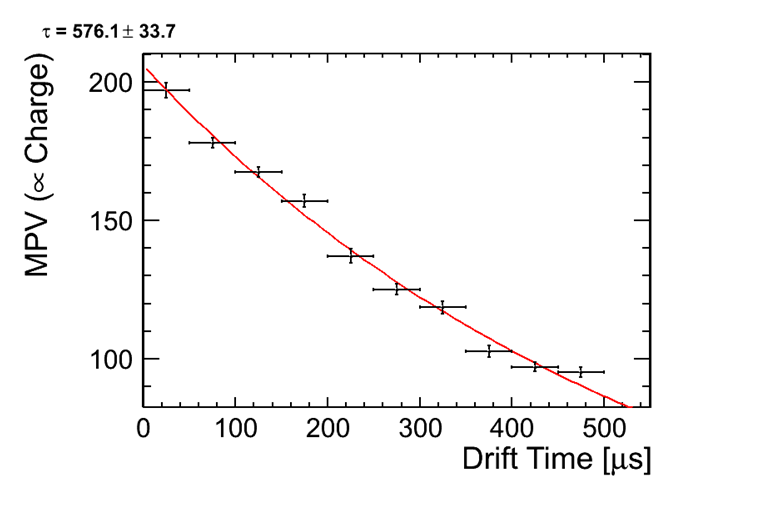
\includegraphics[width=0.45\hsize]{fig/tauExample.eps}
% \end{center}
% \caption{Left: Readout charge as a function of drift time. Readout charge in each drift time bin is fitted by landau function. Right: Average charge readout as a function of drift time which is fitted by exponential to estimate drift electron lifetime.}
% \label{fig:tauExample}
%\end{figure}

\begin{figure}[htbp]
 \begin{center}
  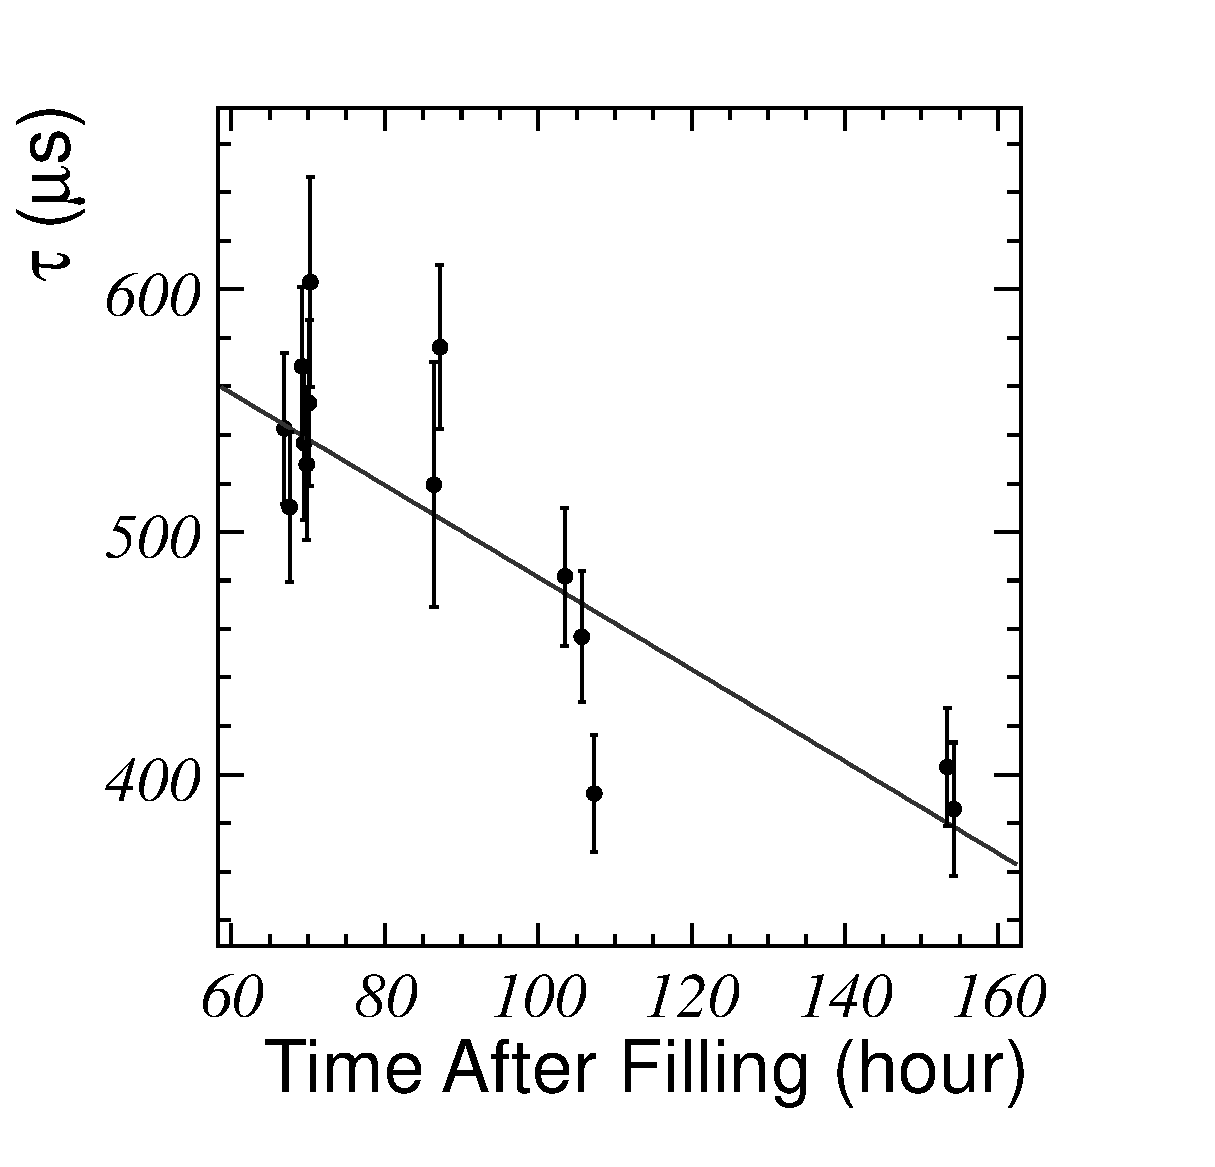
\includegraphics[width=1.0\hsize]{fig/tauHistory.eps}
 \end{center}
 \caption{Drift electron lifetime as a function of duration after initial LAr filling. The lifetime is used to correct the beam data.}
 \label{fig:CosmicPurity}
\end{figure}

\subsection{Signal induction}

For the proper reconstruction and simulation of the signals, the
electronics readout as well as the signal induction on the anode
strips have
to be taken into account. As described above (reference to electronics
section) the shapers of the used charge sensitive preamplifiers have
integration and differentiation time constants of 0.6~$\mu$s and
2.7~$\mu$s, respectively. On the other hand, the signals on the
different strips of the anode are induced by moving electrons,
drifting between the anode-grid and the anode with a drift field of
1~kV/cm. Since this transfer time of about 5~$\mu$s is larger than the
response of the electronics readout, two effects have to be taken into
account: the induced unipolar signal of a strip which collects a
drifting electron becomes broader, compared to the fast electronics
response, whereas on the two neighboring strips, bipolar signals are
induced. Both effects were observed and verified with the weighting
field method, introduced by Shockley \cite{ref:induction}.


%Figure\ref{fig:cross_talk1} shows the signal wave form of stopped channel and the front channel of typical proton event.
%The signal wave form of stopped channel is differential form of the that of the front channel.
%Such signals are appeared at channel number 1 which cannot enter drifted ionization electron in electric power lines.
%One possibility which cause such a phenomenon is following process.
%The distance between anode channels is very short,
%so the influence of mutual capacitance become large
%and this capacitive coupling induce cross talk noise.
%This effect notably appears the channel where the difference of the charge between adjacent channels is large,
%such as the channel around stopped point of proton.
%Then, we implement this phenomenon in Monte Carlo Simulation
%by adding bipolar shape of the signal Gavin shape at adjacent channels.
%The area of the mountain of bipolar shape is 10.5\% of the area of signal Gaussian at each adjacent channel.
%The value of 10.5\% is determined by comparing the hit charge distribution at stopped channel between data and MC simulation.
%Figure\ref{fig:cross_talk2} shows hit charge distribution of stopped channel.
%Black is data and blue is MC simulation with cross talk red is MC simulation without cross talk.
%As fig\ref{fig:cross_talk2} shown, data and MC simulation with cross talk is good agreement,
%so the value of 10.5\% is reasonable.

\begin{figure}[htbp]
  \begin{center}
    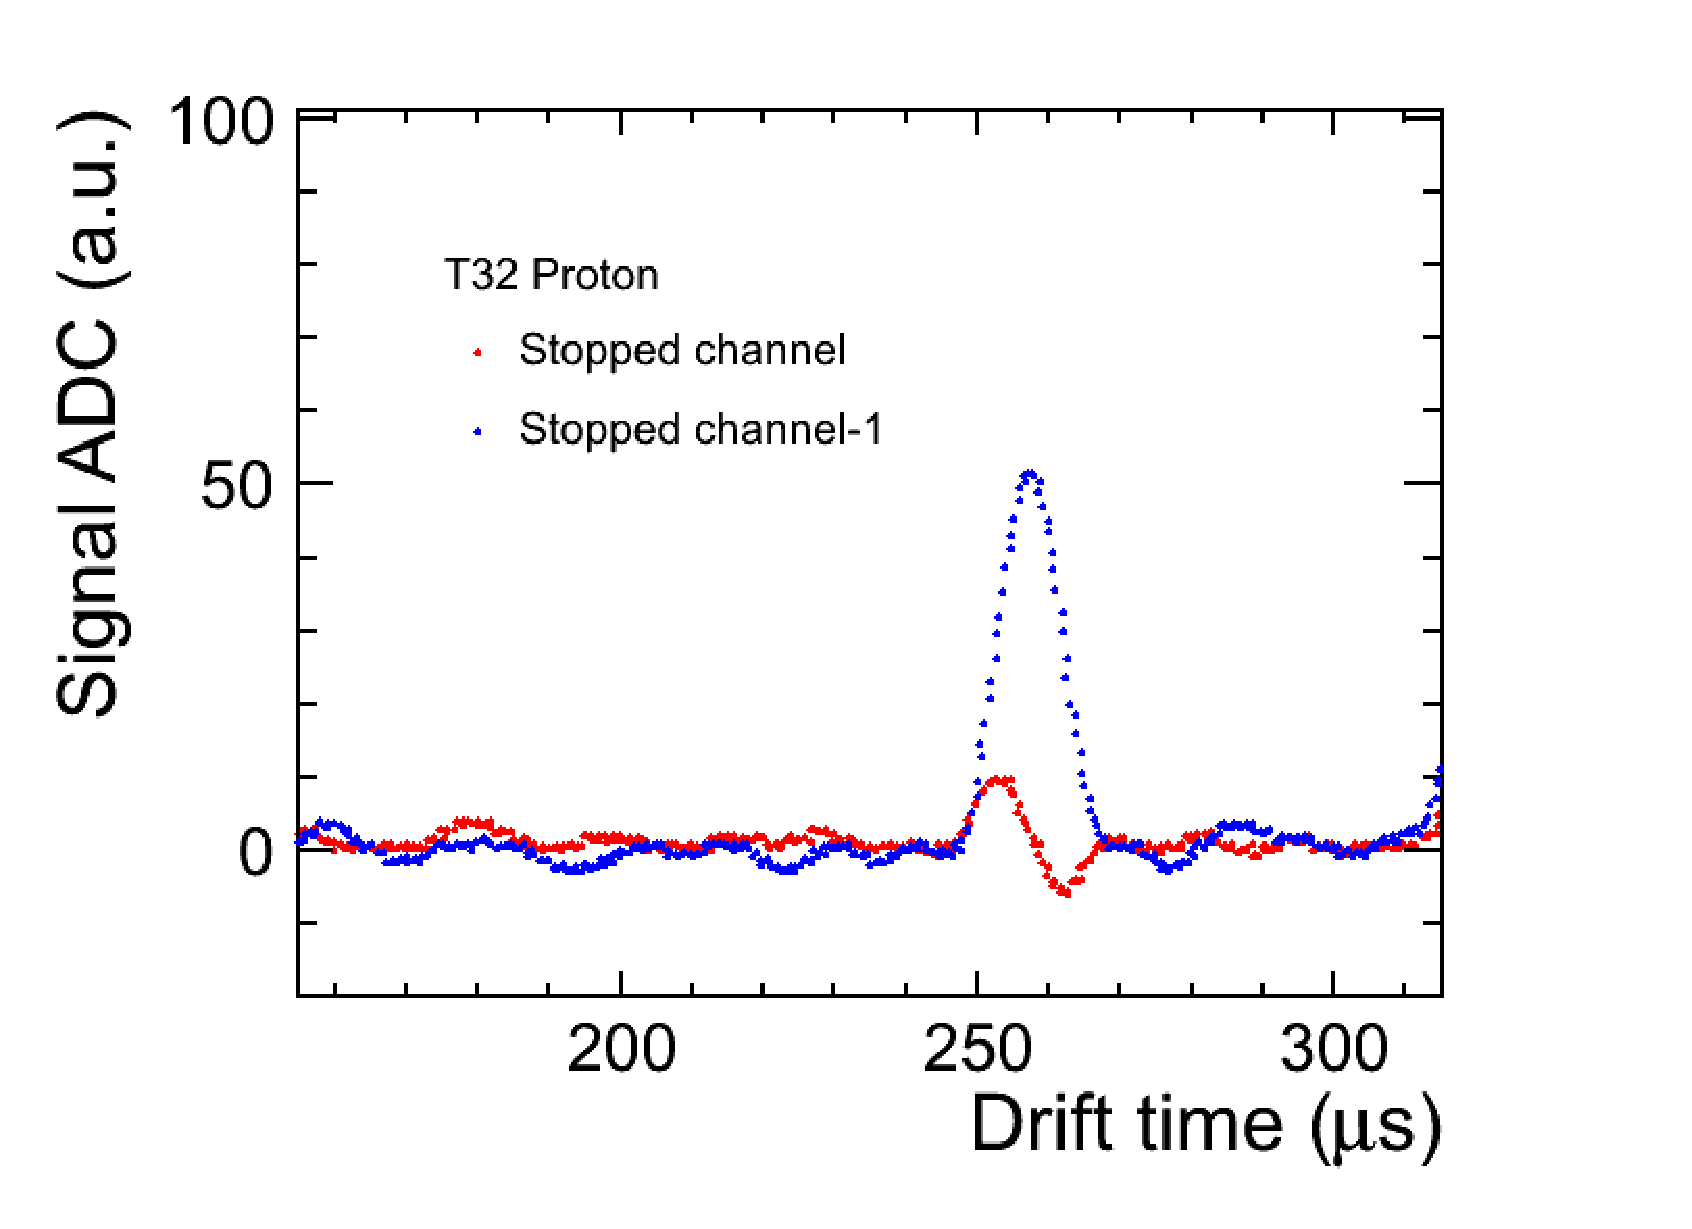
\includegraphics[width=1.0\hsize,clip]{fig/cross_talk_1.eps}
%    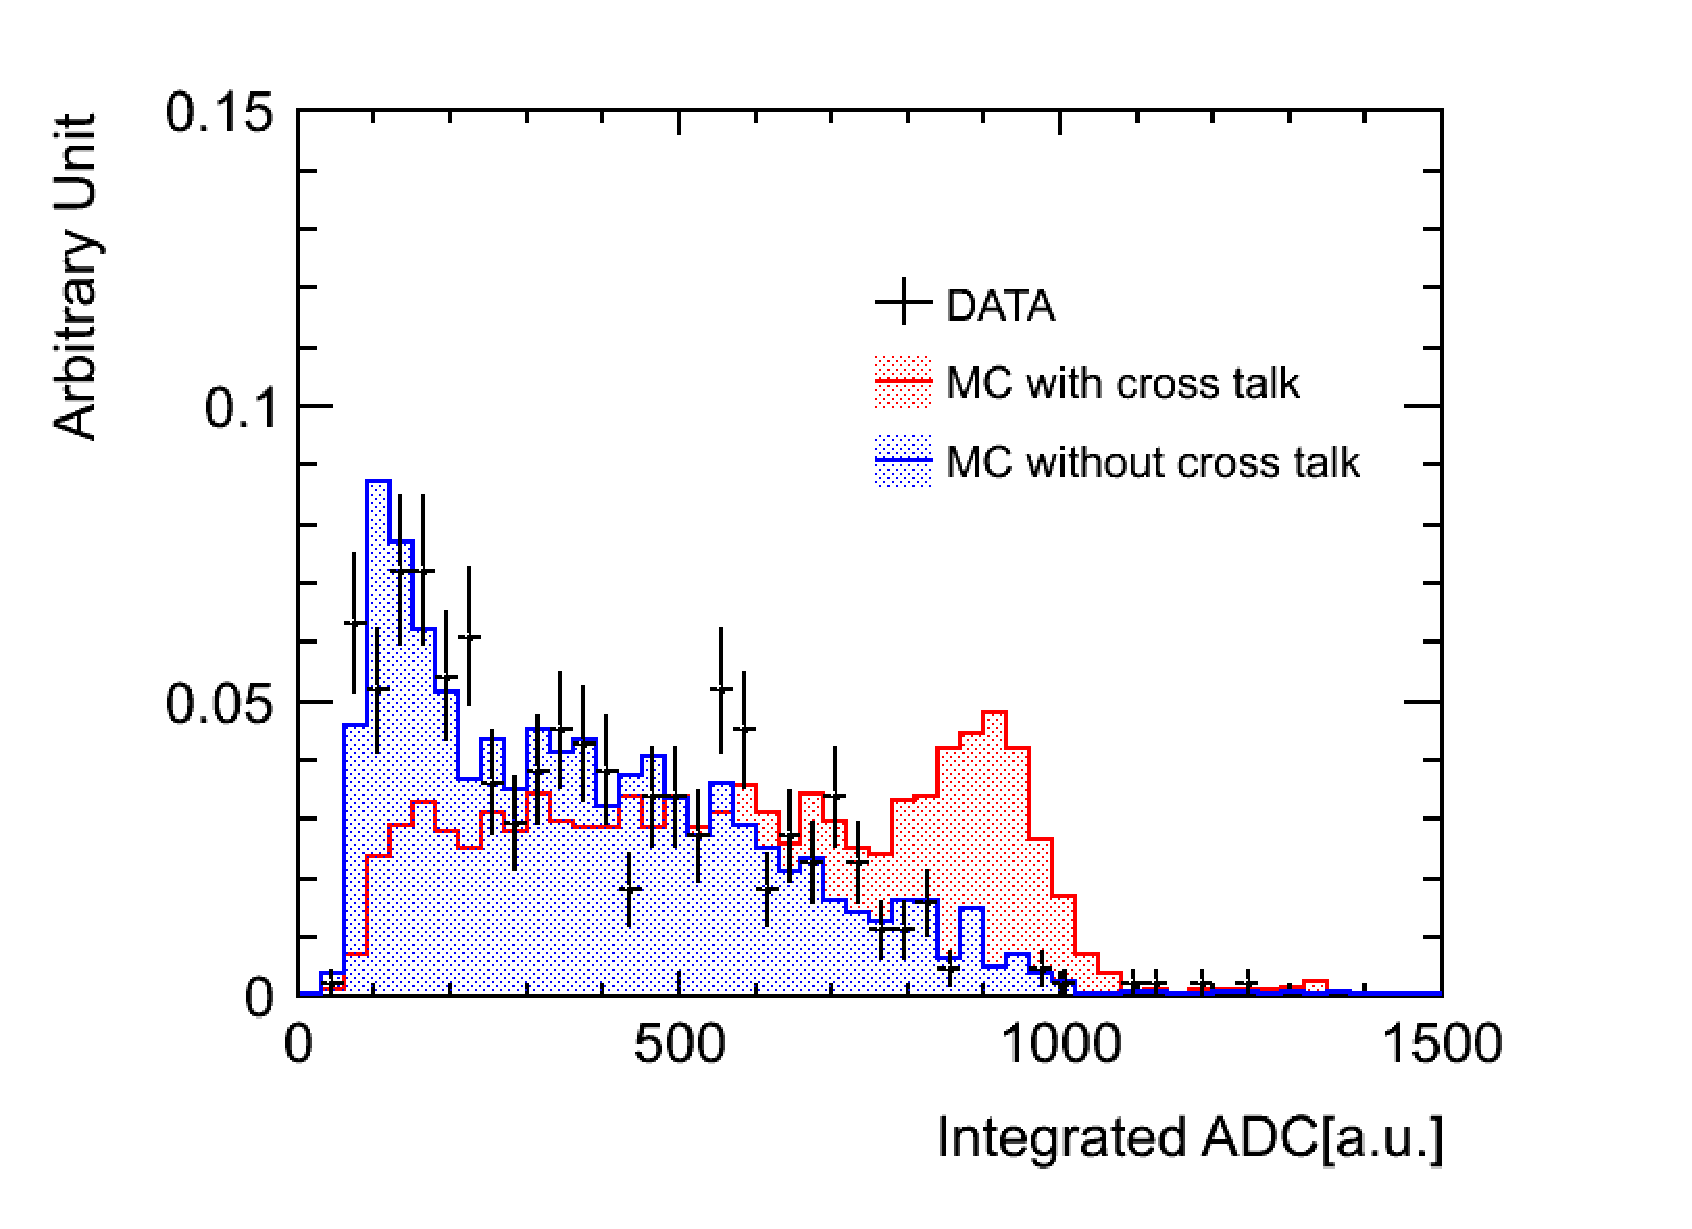
\includegraphics[width=0.45\hsize,clip]{fig/cross_talk_2.eps}
  \end{center}
  \caption{Left plot shows signal wave form of stopped channel and the front channel, 
    and right plot shows hit charge distribution of stopped channel}
  \label{fig:cross_talk1}
  \label{fig:cross_talk2}
\end{figure}


\section{LArTPC Simulation}

Development of the realistic simulation is one of the main task of this experiment.
We try to put several effects (Field distortion, LAr purity, cross talk, etc) into this simulation,
and see if the properties of LArTPC in data can be reproduced using the simulated sample.

\label{Sec:Simulation}
\subsection{Signal Simulation}
GEANT3 is employed for simulating energy deposition of 
initial beam particles and secondary particles to the TPC detector and beam line counters. 
Maximum step of GEANT is set to 0.5 mm which is enough smaller compare to the TPC readout pitch of 1 cm.
Energy cut-off for soft electron/photon emission, which is an important property to understand the
performance of LArTPC, is set to 10 keV. It is minimum possible energy can be set in GEANT3.
After the energy deposition, Recombination of electron and Argon ion is simulated based on the equation (Birks law),
\begin{equation}
  Q = A\frac{Q_{0}}{1+(k/E)\times(dE/dx)\times(1/\rho)}
\label{eq:birkslaw}
\end{equation}
where $Q_{0}$ is initial ionization charge, $\rho$ is density of liquid Argon (=1.4 g/cm$^3$),
$E$ is electric field (V/cm) electric field , and $dE/dx$ is stopping power (Mev/g/cm$^2$).
Parameters of $A$ and $k$ are measured by ICARUS collaboration \cite{658352}.
Electric field is given by 2DFEM calicuration (Fig.\ref{Fig:FieldLine}).

After the recombination, drift of the ionization electrons to anode is simulated
using a simple step simulation with step size of 0.1 mm.
Drift velocity of the ionization electron depends on the liquid Argon temperature,
and the electric field. We use a measurement by ICARUS collaboration \cite{649233}, and
electric field in Fig.\ref{Fig:FieldLine}. Typical drift velocity with 200 V/cm of 
the drift field and temperature of 92K is 0.8 m/ms.
Diffusion of the drift electron is considered and we assume coefficient for the transverse diffusion 
and and lateral diffusion are 9.0 mm$^2$/m and 2.3 mm$^2$/m, respectively (need reference).
\\
**** explanation of diffusion will be skipped **

\begin{itemize}
\item Simulate Signal waveform: Gaussian
\end{itemize}
simulation of recombination, drift, waveform is done for every GEANT step, and
the resulting waveform is summed up for all the particles in the event.
After ending of the event process, noise waveform which describes in the next section is added to the signal waveform,
and then the signal charge is digitized.

%Figure~\ref{Fig:DriftSimulation} shows simulated track of the drift electrons with three different positions.
%left plot with x= 0 mm corresponds to the center of the TPC detector, 
%middle plot with x= 130 mm corresponds to the location of anode grid frame,
%and right plot with x= 350 mm corresponds to the edge of the TPC fiducial.
%Because of the field distortion we find significant displacement of the drift electron in
%x direction for x=130 and x=350. It is a main source of the non-uniformity observed in 
%the through-going pion response (Fig.~\ref{fig:PionQvsCh}).

%\begin{figure}[htbp]
% \begin{center}
%  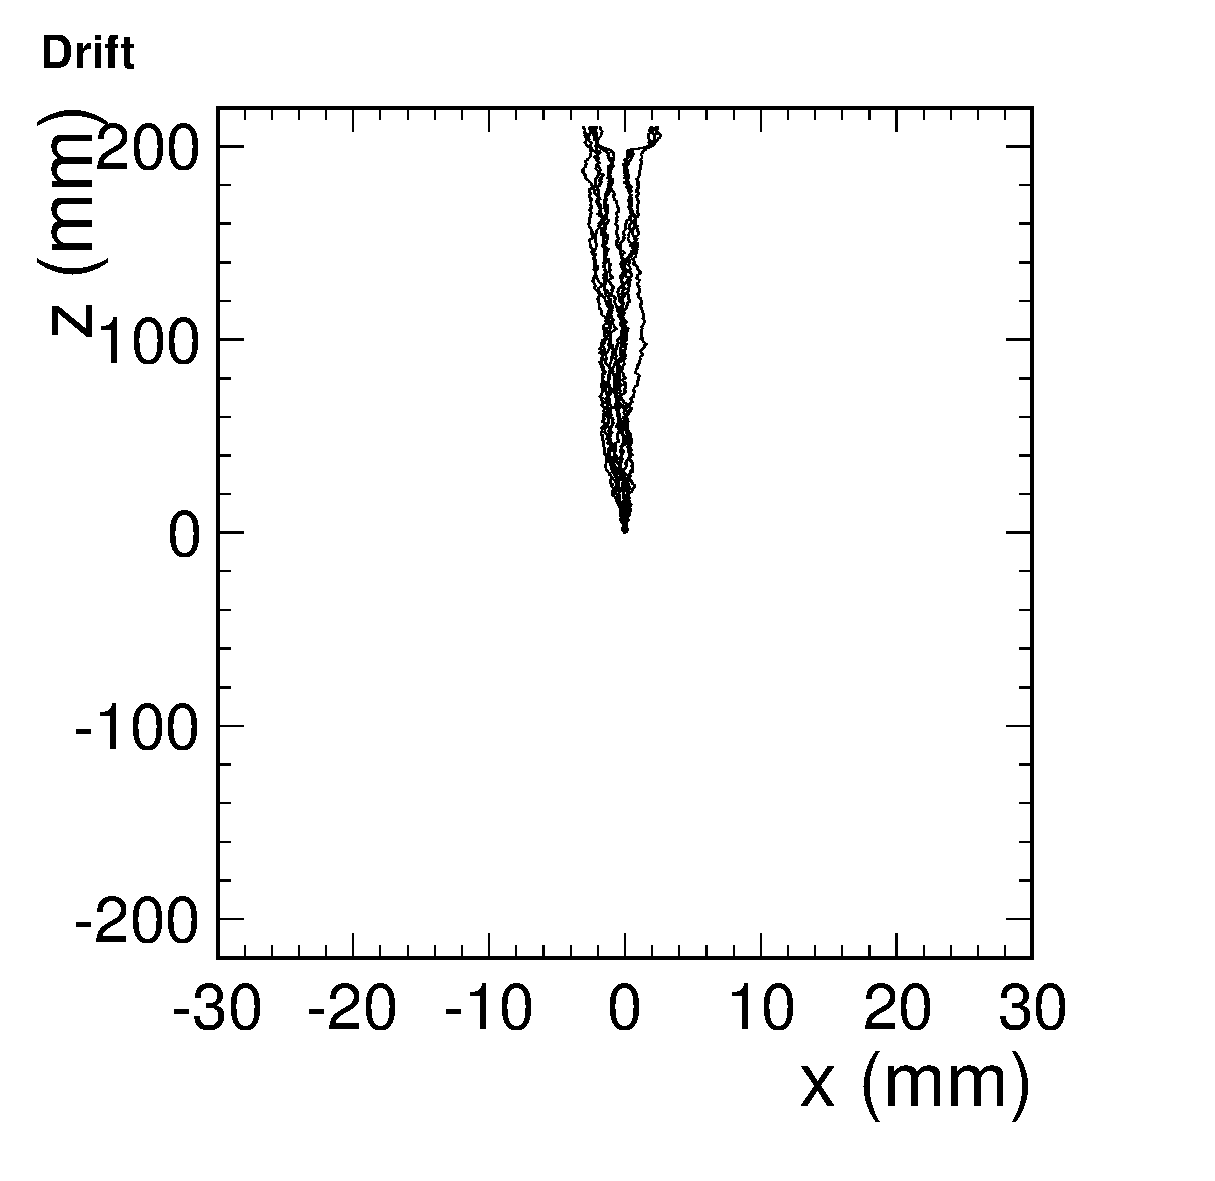
\includegraphics[width=0.3\hsize]{fig/Drift_0.eps}
%  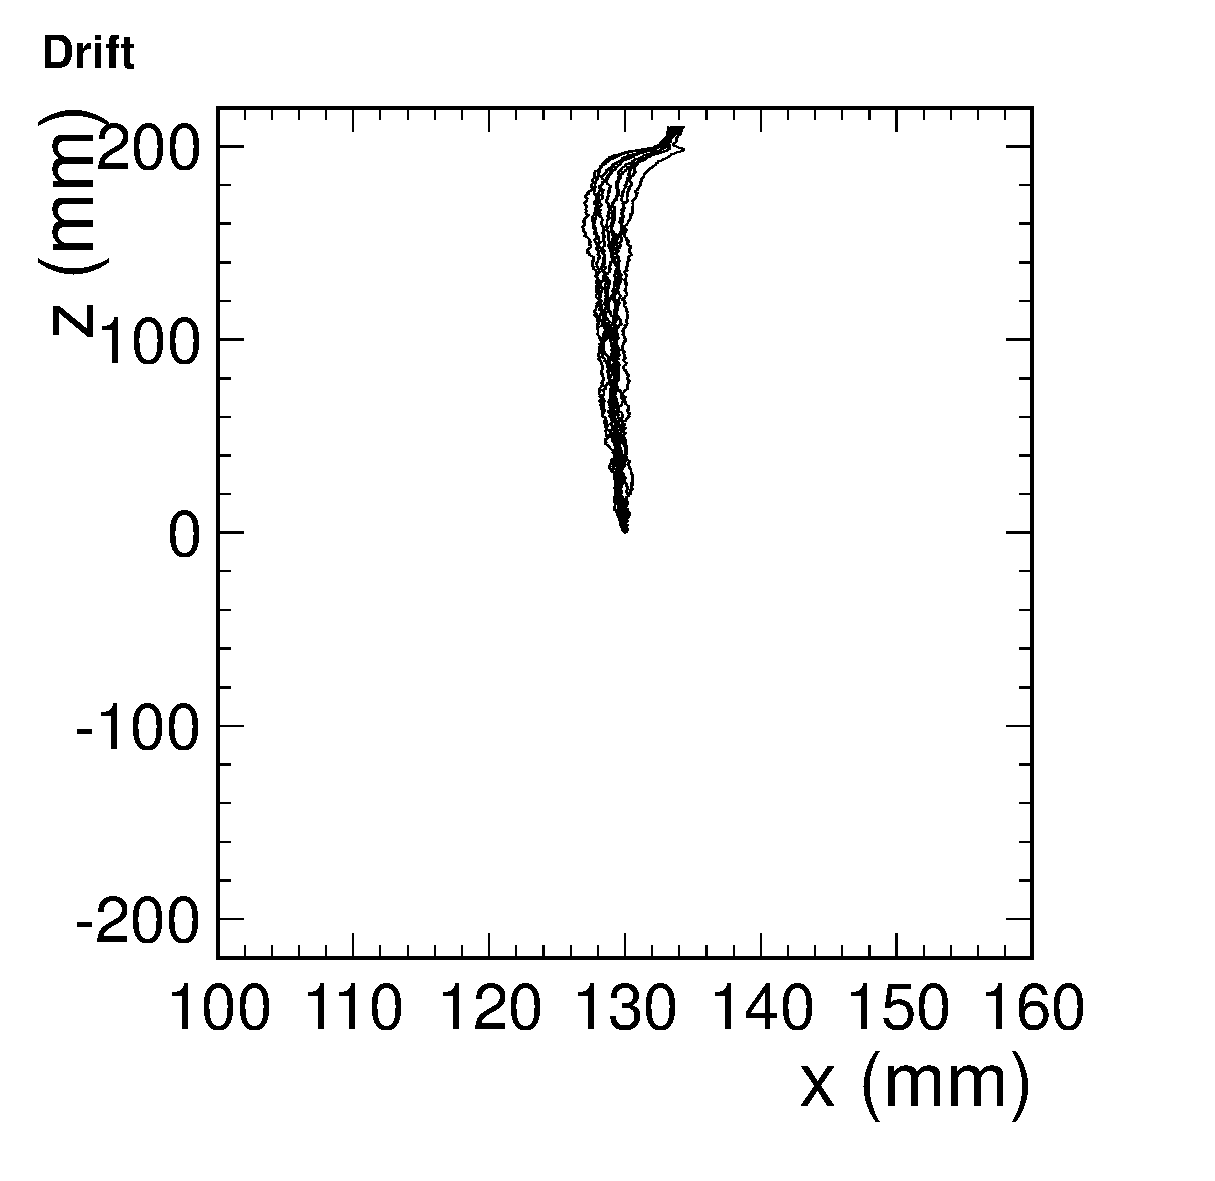
\includegraphics[width=0.3\hsize]{fig/Drift_130.eps}
%  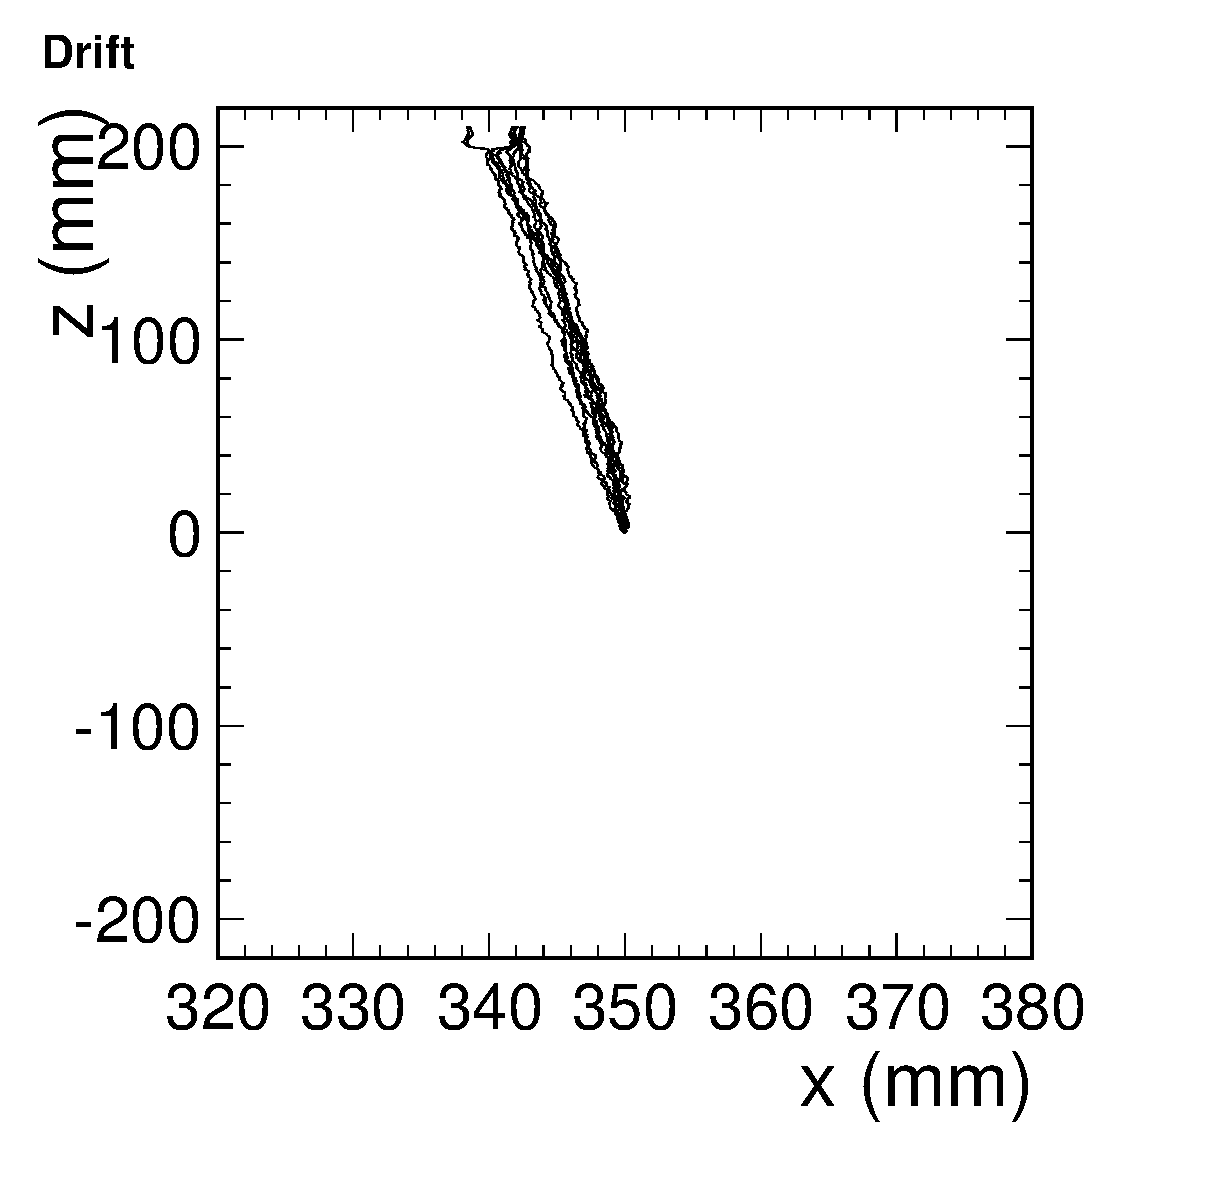
\includegraphics[width=0.3\hsize]{fig/Drift_350.eps}
% \end{center}
% \caption{Simulation of the electron drift with three different initial positions. Left, middle, and right plots corresponds to x=0, x=130 mm, and x=350 mm, respectively.}
% \label{Fig:DriftSimulation}
%\end{figure}

%\begin{itemize}
%\item Plot: drift simulation  (Tanaka)
%\end{itemize}
%\subsection{Preamp Response and Digitization}
%\begin{itemize}
%\item Preamp gain vs channel number  (Naito)
%\end{itemize}

%\subsection{FFT Noise}
%\subsection{FFT Noise}
There are two kinds of noise in the data we obtained, random noise and coherent noise.
Random noise is the noise which exists in each anode channel.
Coherent noise is in each board.
The pseudo noise we implemented in Monte Carlo simulation is composed of random and coherent noise by this reason.

Random noise is generated from FFT(Fast Fourier Transform) distribution of real data. Figure \ref{example10ch} shows an example of FFT distribution.

Coherent noise is generated board by board as the noise scale in the real data we obtained.
The noise scale is defined as a root mean square of pedestal, minimum noise scale is about 3 and maximum noise scale is about 10 in the data.

The ratio of random and coherent noise is 1:1 as equation \ref{PseudoNoise}.
Figure \ref{DATAnoise} shows real data noise and Fig.\ref{MCnoise} shows pseudo noise we implemented in Monte Carlo simulation.
\begin{equation}
  Pseudo\,Noise = \frac{Random\,Noise + Coherent\,Noise}{2}
  \label{PseudoNoise}
\end{equation}

\begin{figure}[!htb]
  \centering
  \centering
  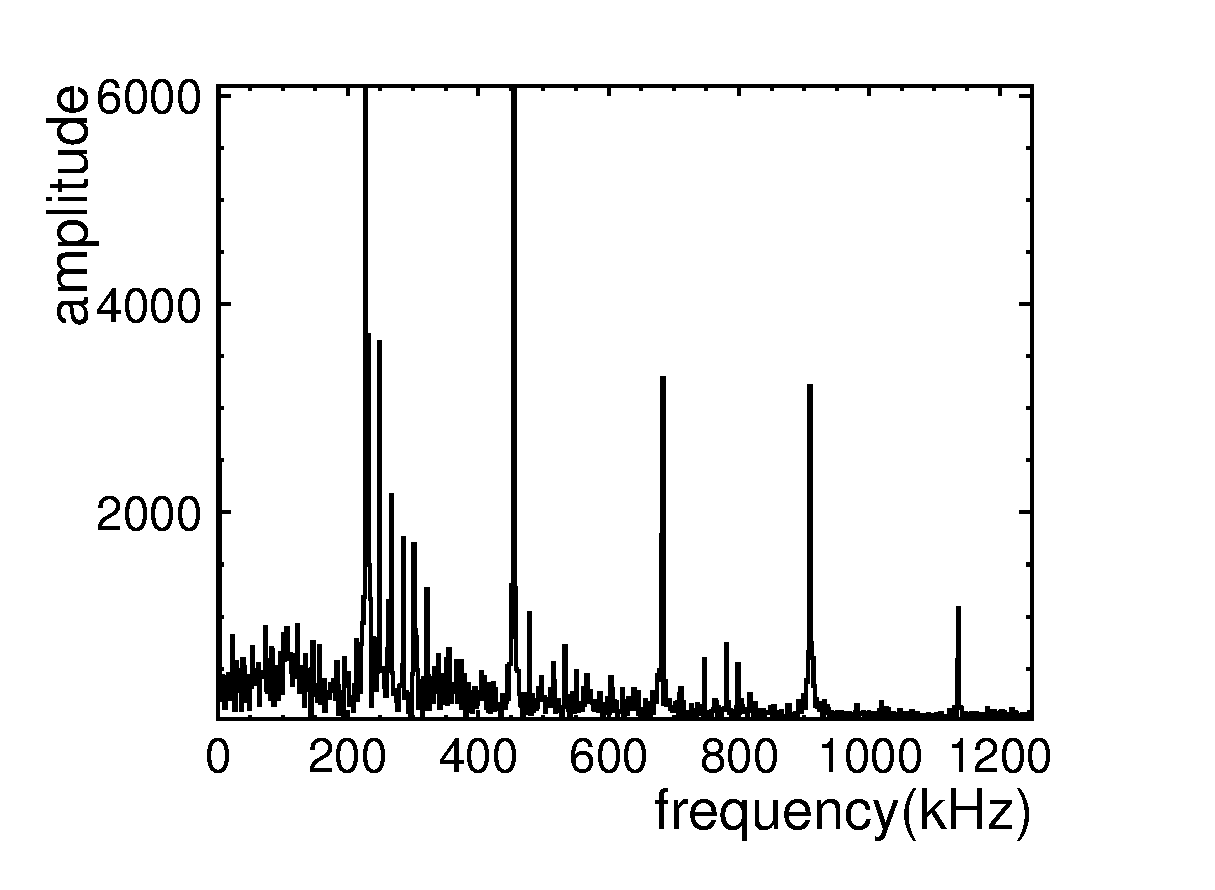
\includegraphics[width=10cm,clip]{./fig/FFTdist.eps}
  \caption{An example distribution of frequency}
  \label{example10ch}
\end{figure}
%\begin{figure}[!htb]
%  \centering
%  \centering
%  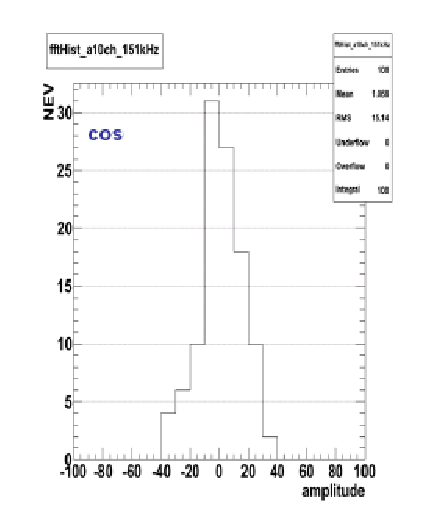
\includegraphics[width=11cm,clip]{./fig/cos.eps}
%  \caption{An example of distribution of amplitude}
%  \label{ampDist}
%\end{figure}
%\begin{figure}[!htb]
%  \centering
%  \centering
%  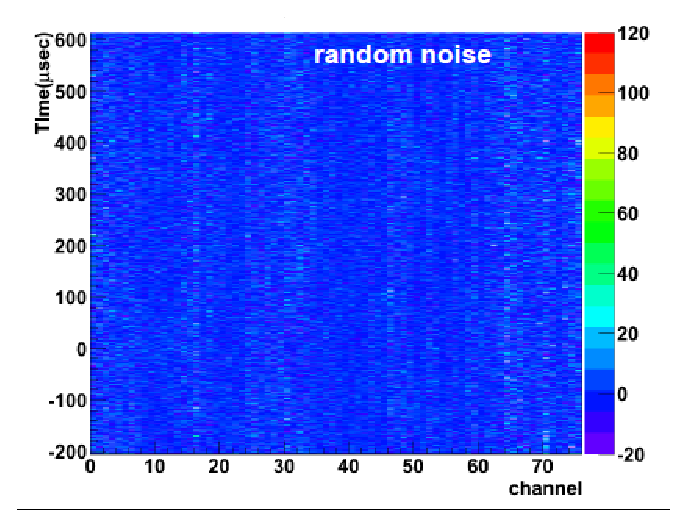
\includegraphics[width=11cm,clip]{./fig/randomnoise.eps}
%  \caption{Random noise}
%  \label{randomNoise}
%\end{figure}
\begin{figure}[!htb]
\begin{minipage}{0.5\hsize}
  \centering
  \includegraphics[width=7cm,clip]{./fig/DATAnoise.eps}
  \caption{Data noise}
  \label{DATAnoise}
\end{minipage}
\begin{minipage}{0.5\hsize}
  \centering
  \includegraphics[width=7cm,clip]{./fig/MCnoise.eps}
  \caption{Pseudo noise(Noise simulation)}
  \label{MCnoise}
\end{minipage}
\end{figure}
%\begin{figure}[!htb]
%  \centering
%  \centering
%  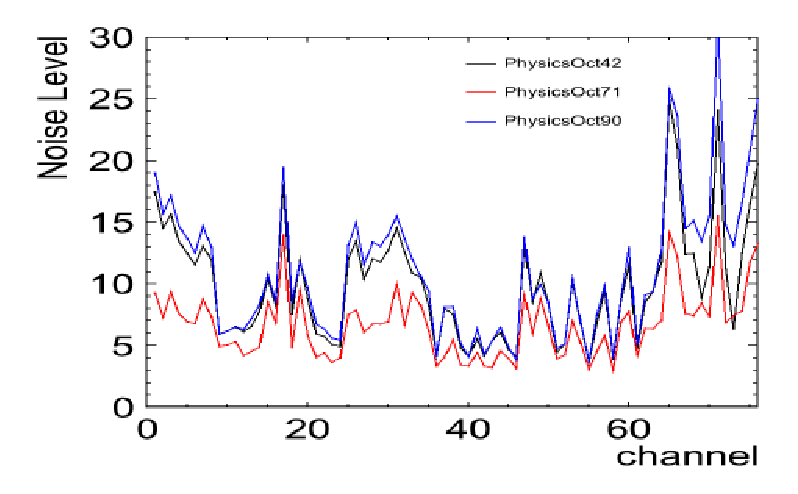
\includegraphics[width=11cm,clip]{./fig/scaling.eps}
%  \caption{Noise level}
%  \label{scaling}
%\end{figure}
\subsection{Noise Simulation}

\begin{itemize}
\item We generate noise from FFT amplitude distribution such as in Fig.\ref{Fig:FFT}
\item By using empty event, prepare template distribution of amplitude for each channel and each frequency bin
\item Obtain waveform by generating random number from the template
\item Coherent noise is added board by board
\end{itemize}

%There are two kinds of noise in the data we obtained, random noise and coherent noise.
%Random noise is the noise which exists in each anode channel.
%Coherent noise is in each board.
%The pseudo noise we implemented in Monte Carlo simulation is composed of random and coherent noise by this reason.

%Random noise is generated from FFT distribution of real data (See Fig.\ref{fig:FFT}).

%Coherent noise is generated board by board as the noise scale in the real data we obtained.
%The noise scale is defined as a root mean square of pedestal, minimum noise scale is about 3 and maximum noise scale is about 10 in the data.

%The ratio of random and coherent noise is 1:1 as equation \ref{PseudoNoise}.
%Figure \ref{DATAnoise} shows real data noise and Fig.\ref{MCnoise} shows pseudo noise we implemented in Monte Carlo simulation.
%\begin{equation}
%  Pseudo\,Noise = \frac{Random\,Noise + Coherent\,Noise}{2}
%  \label{PseudoNoise}
%\end{equation}

%\begin{figure}[!htb]
%  \centering
%  \centering
%  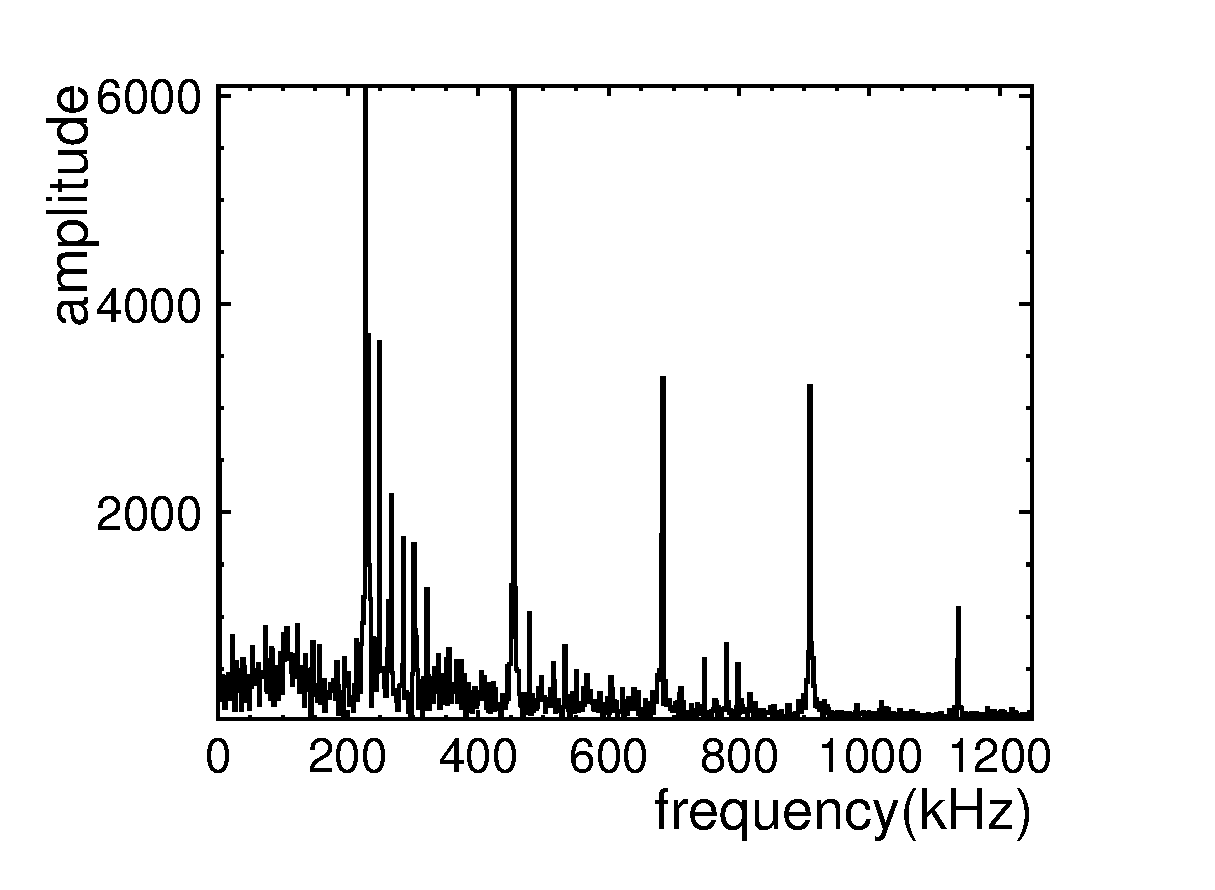
\includegraphics[width=10cm,clip]{./fig/FFTdist.eps}
%  \caption{An example distribution of frequency}
%  \label{example10ch}
%\end{figure}
%\begin{figure}[!htb]
%  \centering
%  \centering
%  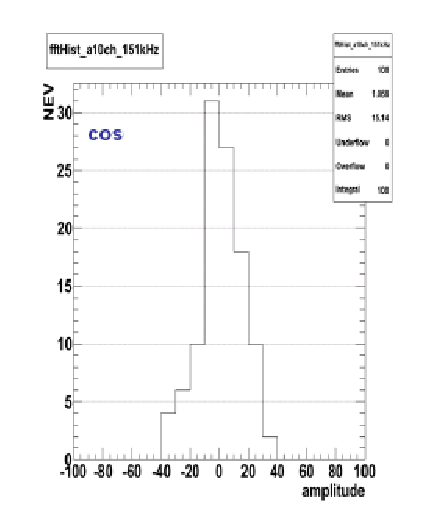
\includegraphics[width=11cm,clip]{./fig/cos.eps}
%  \caption{An example of distribution of amplitude}
%  \label{ampDist}
%\end{figure}
%\begin{figure}[!htb]
%  \centering
%  \centering
%  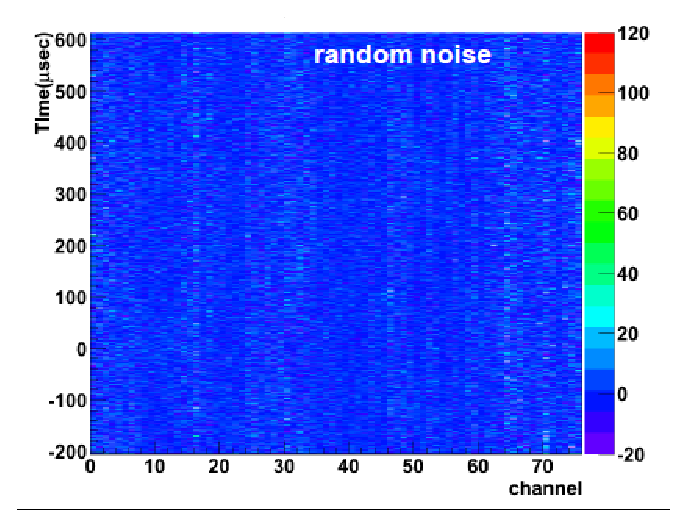
\includegraphics[width=11cm,clip]{./fig/randomnoise.eps}
%  \caption{Random noise}
%  \label{randomNoise}
%\end{figure}
%\begin{figure}[!htb]
%  \begin{center}
%    \includegraphics[width=0.45\hsize,clip]{./fig/DATAnoise.eps}
%    \includegraphics[width=0.45\hsize,clip]{./fig/MCnoise.eps}
%  \end{center}
%  \caption{Noise}
%  \label{DATAnoise}
%  \label{MCnoise}
%\end{figure}
%\begin{figure}[!htb]
%  \centering
%  \centering
%  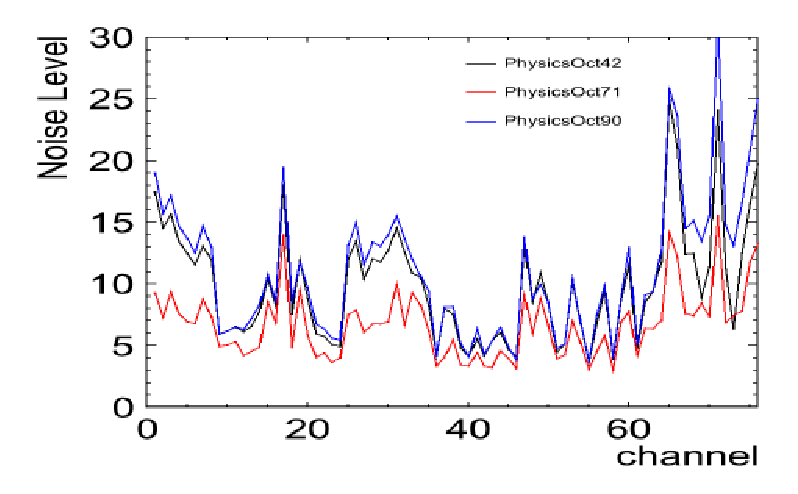
\includegraphics[width=11cm,clip]{./fig/scaling.eps}
%  \caption{Noise level}
%  \label{scaling}
%\end{figure}

Figure~\ref{Fig:SimulatedKaon} shows simulated event of 630 MeV/$c$ $K^+\to\mu\nu$.

\begin{figure}[htbp]
 \begin{center}
  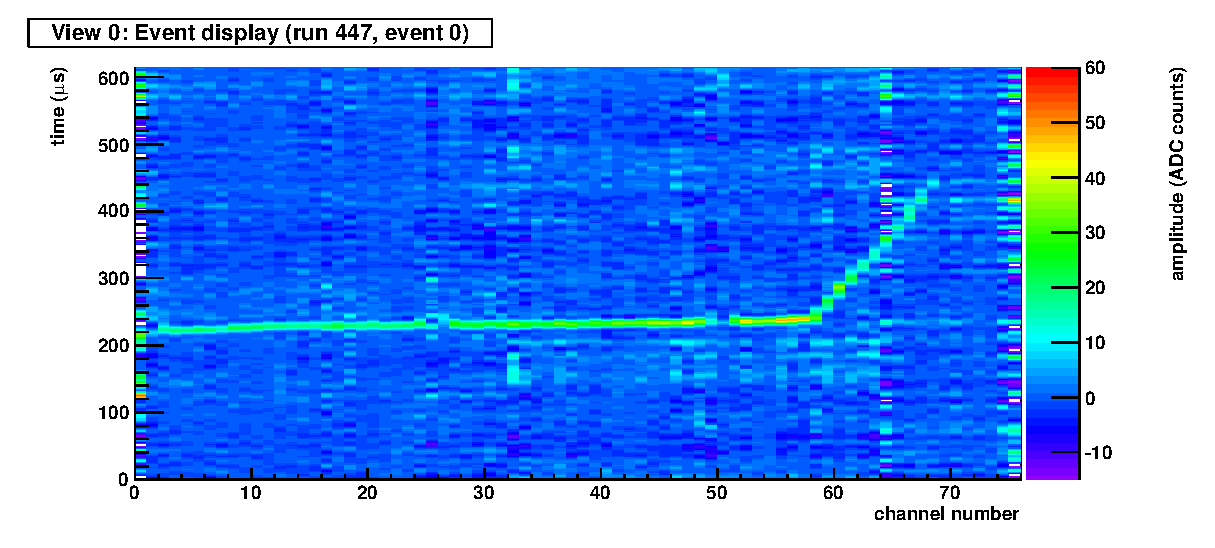
\includegraphics[width=0.8\hsize]{fig/Simulation.eps}
 \end{center}
 \caption{Event display of simulated events for 630 MeV/$c$ $K^+$.}
 \label{Fig:SimulatedKaon}
\end{figure}

\begin{itemize}
\item Explain Landau distribution ("bare" track and "dressed" track)
\item pion track (800 MeV/c) and soft electron ($\sim$10 keV) has different $dE/dx$ = recombination
\item Set delta-ray cut off = 10 keV in simulation, and take ICARUS measurement of recombination.
\item Hit charge distribution is in good agreement between data and MC.
\end{itemize}

\begin{figure}[htbp]
 \begin{center}
  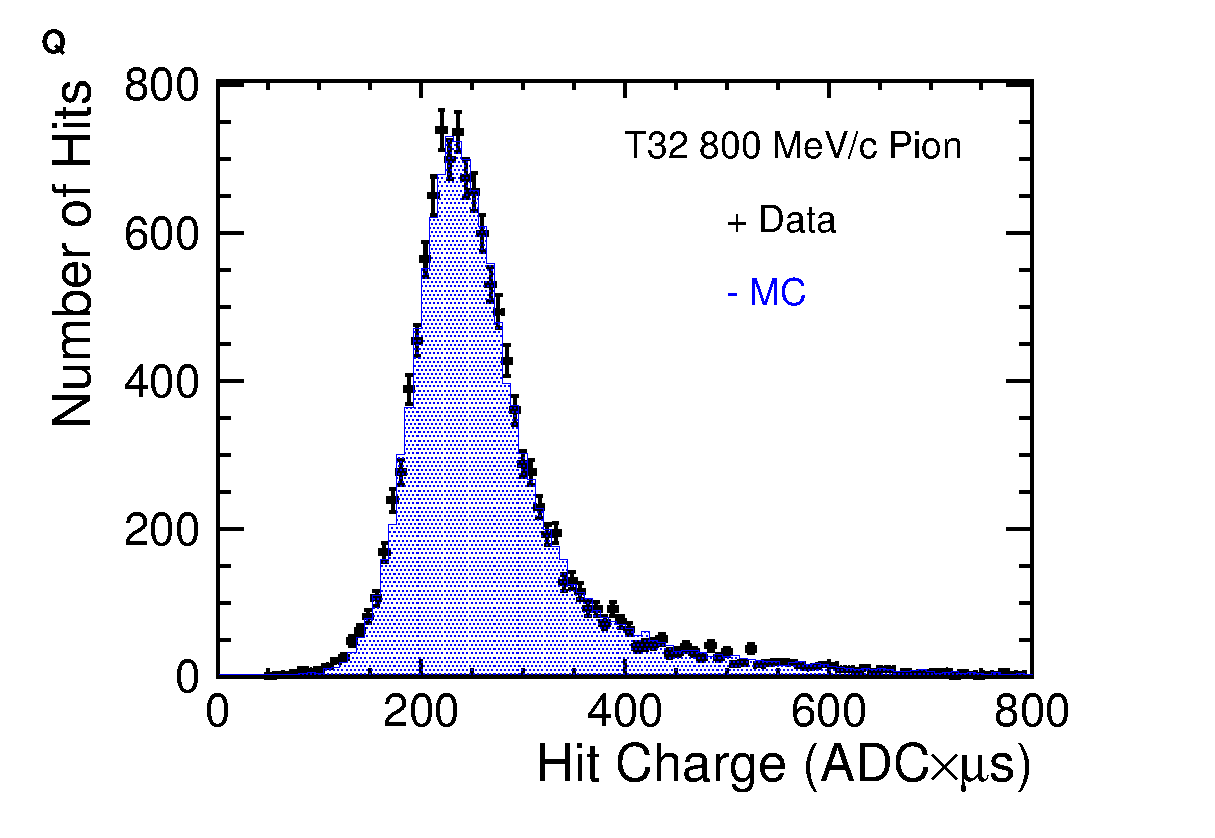
\includegraphics[width=0.8\hsize]{fig/PionLandau.eps}
 \end{center}
 \caption{Hit charge distribution for 800 MeV/c through-going $\pi^+$ sample. Points and histograms correspond to data and MC, respectively}
 \label{Fig:PionLandau}
\end{figure}


%\subsection{Beam energy}
We estimated a beam momentum using simple MC simulation.
Figure \ref{K11Br_Beam_line} shows MC simulation's geometry.
We generate 800MeV/$c$ pencil beam and shoot the beam downstream.
Figure \ref{k_pi_momentum} shows Kaon and Pion momentum distribution
using this MC simulation at BDC.
Kaon beam momentum is estimated by the momentum distribution of MC simulation.
%Actually, kaon momentum distribution peak is adjusted so that kaon decay point of MC simulation is consistent with data.
%Section \ref{kaon_energy_section} explains this point.
%And proton momentum is estimated in other way, using TREK detector TOF information.
%Section \ref{proton_energy_section} shows proton momentum distribution.

\begin{figure}[!htb]
  \centering
  \centering
  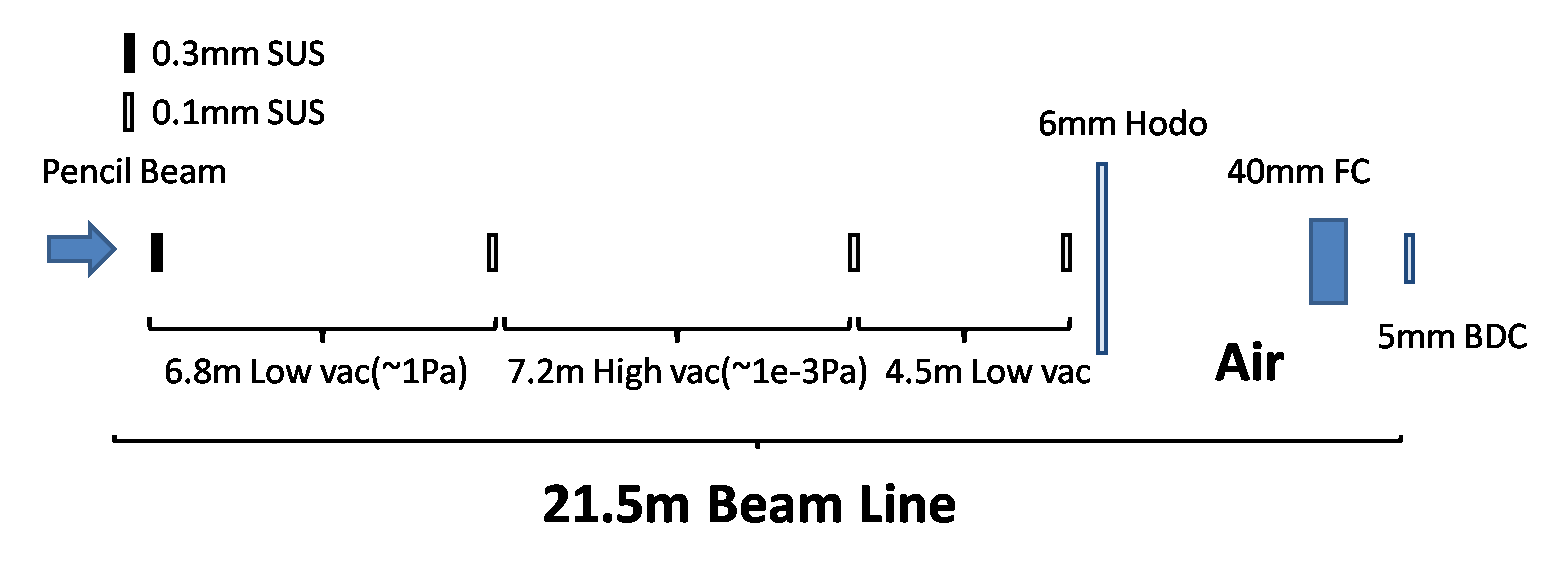
\includegraphics[width=10cm,clip]{./fig/K11Br_beamline_sim.eps}
  \caption{K1.1 Br beam line}
  \label{K11Br_Beam_line}
\end{figure}


\begin{figure}[!htb]
  \centering
  \centering
  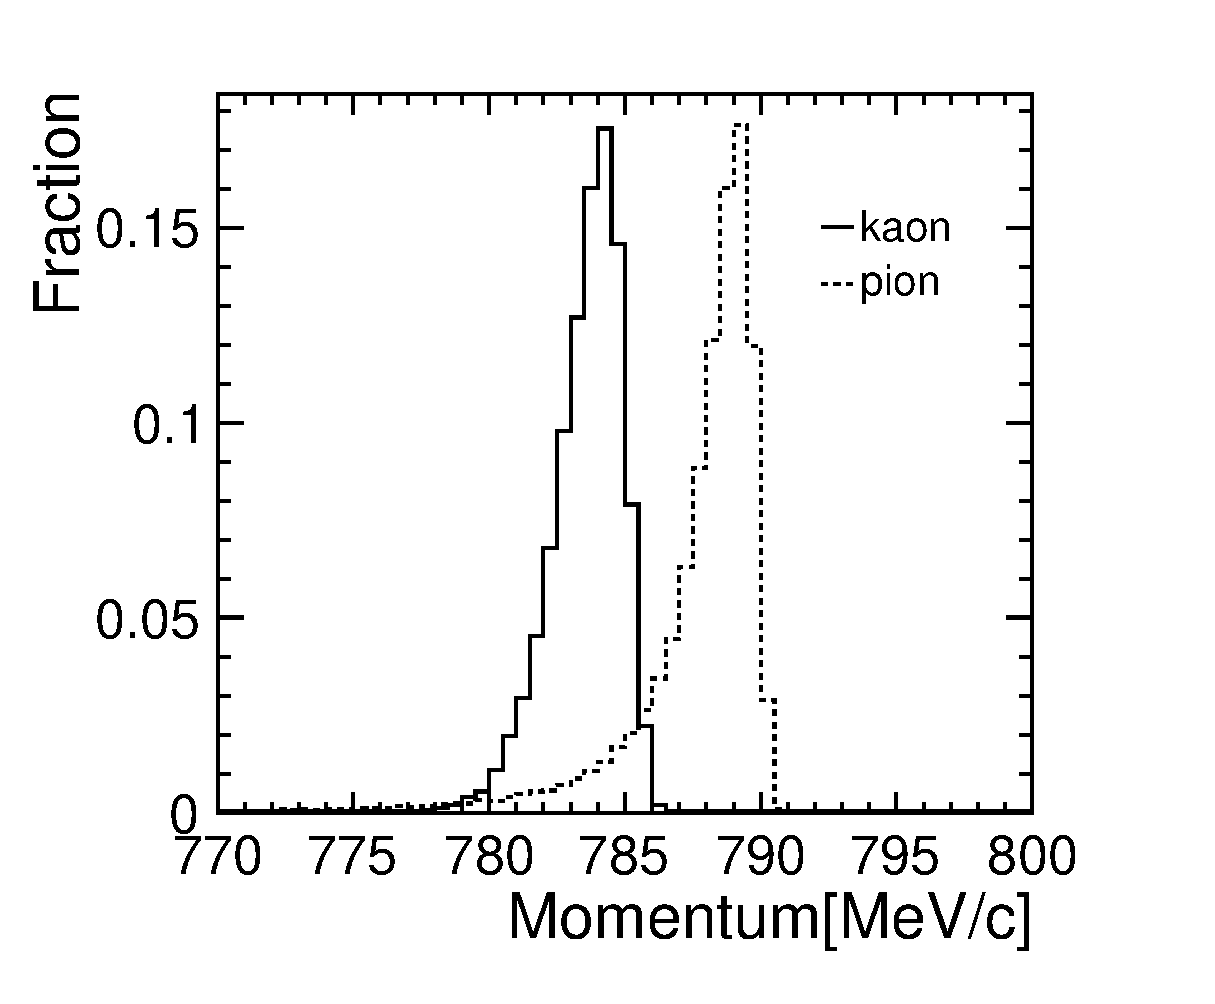
\includegraphics[width=10cm,clip]{./fig/Kaon_pion_momentum_nogrid.eps}
  \caption{Kaon and Pion momentum distribution at BDC}
  \label{k_pi_momentum}
\end{figure}


\subsubsection{Kaon energy
  \label{KaonEnergy}
}
Kaon beam momentum is estimated by the momentum distribution of MC simulation.
We change Kaon beam momentum in a range of 700 - 800 MeV/$c$ and search the momentum that decay point distribution of MC simulation is consistent with data one.

\subsubsection{Proton energy}
Proton momentum shown in Figure \ref{fig:Proton_momentum} is used as proton beam momentum of MC simulation.

\subsubsection{Energy deposition in degrader}
It is too high energy that Kaon beam stops in the fiducial volume of 250LAr TPC.
In order to degrade the beam momentum, some lead glass blocks and a lead brick were inserted in front of 250LAr TPC as degrader.
%We estimate energy deposition in degrader by using MC simulation.
Figure \ref{energy_deposition} shows energy deposition distribution in degrader.


\begin{figure}[!htb]
  \centering
  \centering
  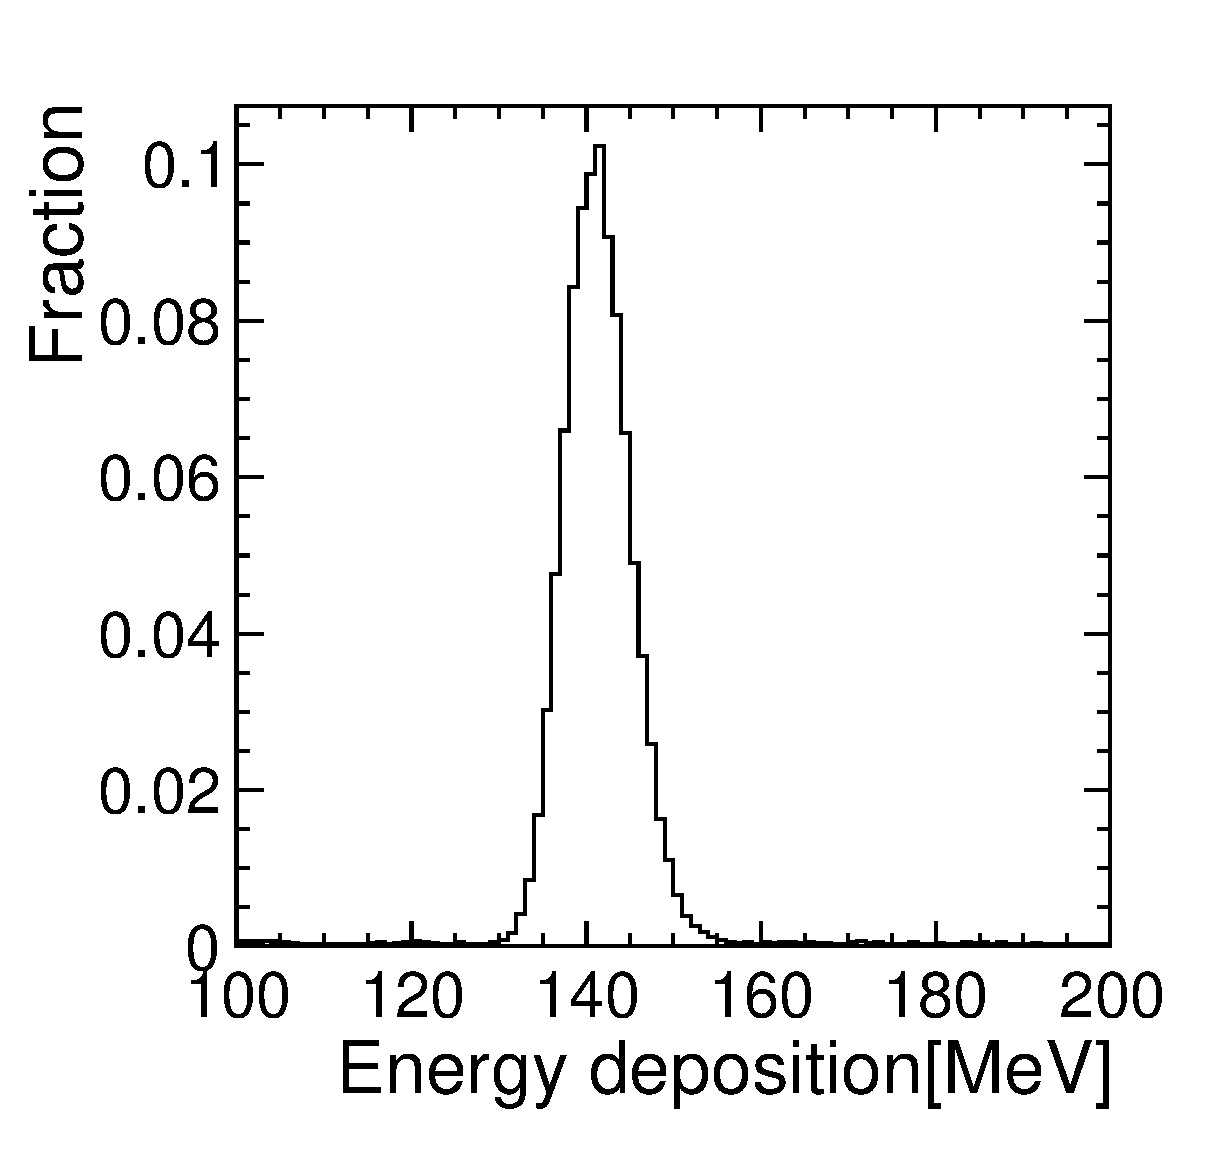
\includegraphics[width=10cm,clip]{./fig/energy_deposition.eps}
  \caption{Energy deposition in degrader}
  \label{energy_deposition}
\end{figure}





